\RequirePackage{fix-cm}
\documentclass[twocolumn]{svjour3}
\smartqed
\journalname{Proc.\ VLDB Endow.}

\usepackage[T1]{fontenc}
\usepackage[utf8]{inputenc}
\usepackage{lmodern}
\usepackage{microtype}
\usepackage{amsmath,amssymb,amsfonts}
\usepackage{graphicx}
\usepackage{booktabs}
\usepackage{multirow}
\usepackage{array}
\usepackage{xcolor}
\usepackage{url}
\usepackage{xurl}
\usepackage{listings}
\usepackage{algorithm}
\usepackage{algpseudocode}
\usepackage{enumitem}
\usepackage[hidelinks]{hyperref}
\usepackage[numbers,sort&compress]{natbib}
\makeatletter\let\cl@chapter\@empty\makeatother
\usepackage[capitalize,noabbrev]{cleveref}

\hypersetup{
  pdftitle={DRL: Deterministic Relational Middleware for Transaction-Safe Enterprise NL2SQL},
  pdfauthor={Sanjay Mishra and Divya Chukkapalli and Ganesh R. Naik}
}

\lstdefinelanguage{Python3}{
  morekeywords={import,from,def,class,return,if,else,elif,for,while,try,except,with,as,True,False,None},
  sensitive=true,
  morecomment=[l]{\#},
  morestring=[b]",
}

\lstset{
  language=Python3,
  basicstyle=\footnotesize\ttfamily,
  keywordstyle=\color{blue!80!black}\bfseries,
  commentstyle=\color{gray}\itshape,
  stringstyle=\color{green!60!black},
  breaklines=true,
  frame=single,
  rulecolor=\color{gray!40},
  backgroundcolor=\color{gray!5},
  numbers=left,
  numberstyle=\tiny\color{gray},
  numbersep=5pt,
  xleftmargin=1em
}

\spnewtheorem{drdef}{Definition}{}{\itshape}
\spnewtheorem{drthm}{Theorem}{}{\itshape}

\begin{document}

\title{DRL: A Deterministic Relational Middleware Layer for\\Transaction-Safe Enterprise NL2SQL Under Schema-Graph Scaling}

\titlerunning{DRL: Deterministic Relational Middleware for Enterprise NL2SQL}

\author{Sanjay Mishra\thanks{Corresponding author.} \and Divya Chukkapalli \and Ganesh R. Naik}

\authorrunning{Mishra et al.}

\institute{%
  Sanjay Mishra \at Fidelity Investments; Independent Researcher; Raleigh, NC, USA \\
  \email{sanmish4@icloud.com}
  \and
  Divya Chukkapalli \at Microsoft; Independent Researcher; Apex, NC, USA \\
  \email{divya.95j@gmail.com}
  \and
  Ganesh R. Naik \at College of Medicine and Public Health, Flinders University; Bedford Park, SA, Australia \\
  \email{ganesh.naik@flinders.edu.au}
}

\date{}

\maketitle

% =============================================================================
\section*{Abstract}
% =============================================================================

Deploying natural-language interfaces over enterprise OLTP catalogs fails at production scale because unconstrained semantic parsers collapse under \emph{schema-graph scaling}: hundreds of normalized tables, partial foreign-key enforcement, and namespace ambiguity inflate schema context beyond stable LLM attention budgets.
We present \textbf{DRL} (\emph{Deterministic Relational Layer}), a middleware architecture interposing a transaction-safe pipeline between conversational front-ends and ANSI-oriented SQL backends (PostgreSQL and MySQL evaluated; SQL Server supported in the emitter specification).
DRL comprises \emph{dynamic context pruning} (implemented), \emph{relational AST compilation} (specified with dialect emitter), and \emph{transactional safeguard verification} (implemented via EXPLAIN gating and NULL guards), together bounding context and flagging operational silent divergence ($\text{SD}_{\text{op}}$).
We contribute (i)~a formal OLTP schema-graph scaling model, (ii)~a 1{,}000-pair Workload Verification Suite and open harnesses, (iii)~measured middleware baselines B0--B3, and (iv)~a structural failure taxonomy on enterprise NL2SQL.
On PostgreSQL, DRL reduces injected schema context by \textbf{71\%} (B1$\rightarrow$B2) at pruning \textbf{p95\,=\,0.76\,ms} and middleware \textbf{p95\,=\,4.1\,ms} (excluding LLM).
GPT-4o, Gemini~2.5, and Claude Sonnet~4.5 achieve \textbf{51.6\%}, \textbf{50.1\%}, and \textbf{46.5\%} execution match on the suite; $\text{SD}_{\text{op}}$ flags \textbf{88--99\%} of EX-passing queries.
GPT-4o EX failures are dominated by semantic/projection errors (\textbf{391/483}), not invalid column names (\textbf{0 ORA-00904}).
DRL reframes enterprise NL2SQL as systems engineering---context bounding, verification, and plan-aware admission---not a leaderboard exercise.

\keywords{OLTP middleware \and NL2SQL \and schema-graph scaling \and silent semantic divergence \and query plan safety \and multi-dialect compilation}

% =============================================================================
\section{Introduction}
\label{sec:intro}
% =============================================================================

Natural-language-to-SQL (NL2SQL) systems report 85--91\% execution accuracy on academic benchmarks whose schemas average fewer than six tables with complete foreign-key documentation~\cite{yu2018spider,li2023can}.
When the same model families are deployed against production OLTP catalogs---150--500 highly normalized tables, legacy abbreviations, duplicated column names across unrelated domains, and foreign keys that exist in application logic but not in catalog metadata---reported accuracy drops \textbf{30--40 percentage points} relative to Spider-class evaluations.
This degradation is not primarily a ``model capacity'' phenomenon; it is a \emph{systems boundary} phenomenon: the parser receives an exponentially growing structural search space without a deterministic mechanism to bound it, compile it, or verify that emitted SQL preserves transactional semantics under concurrent write load.

We formalize this as the \textbf{OLTP Schema Graph Scaling Problem}.
Let $G=(V,E)$ denote the enterprise catalog graph where $V$ is the set of base relations and $E\subseteq V\times V$ encodes declared or inferred join paths (foreign keys, shared surrogate keys, and application-enforced links).
For a natural-language intent $q$, naive NL2SQL selects a SQL program $\hat{s}$ by conditioning an LLM on the full schema $\mathcal{S}(G)$---typically $|V|>150$ in Tier~2/3 domains.
The probability of selecting a relation subset $V_q\subset V$ that supports a semantically correct query scales poorly with $|V|$ because (i) column-name collisions inflate the effective vocabulary, (ii) dropped FK constraints remove graph sparsity that humans rely on for join disambiguation, and (iii) LLM context windows treat $\mathcal{S}(G)$ as unstructured text rather than as a typed join hypergraph with cardinality constraints.

\textbf{Our thesis.} Enterprise NL2SQL requires a \emph{Deterministic Relational Middleware Layer} (DRL) that:
\begin{enumerate}[label=(\roman*)]
  \item \textbf{Bounds context} before generation by extracting a minimal join-safe sub-graph $G_q=(V_q,E_q)$ with $|V_q|\le k$ (we use $k{=}5$).
  \item \textbf{Compiles} LLM output through an ANSI-first Relational AST (RAST) so dialect emission is a pure backend mapping, not an LLM responsibility.
  \item \textbf{Verifies} each candidate query against operational divergence ($\text{SD}_{\text{op}}$) and physical plan safety before execution on hot OLTP paths.
\end{enumerate}

\textbf{Contributions.}
\begin{enumerate}[label=(\arabic*)]
  \item Formalization of the OLTP schema-graph scaling problem and context scaling degradation ($\Delta_{\text{CSD}}$; \Cref{sec:problem}).
  \item DRL middleware architecture with implemented pruning router and safeguard layer, plus specified RAST/dialect emitter (\Cref{sec:arch}).
  \item A 1{,}000-pair Workload Verification Suite (333/334/333 per tier) with reproducible harnesses (\Cref{sec:harness,sec:artifact}).
  \item Measured middleware baselines B0--B3 and NL2SQL evaluation on PostgreSQL/MySQL, including structural failure taxonomy (\Cref{sec:eval,sec:failures}).
\end{enumerate}

The verification suite is a \emph{stress harness}, not a leaderboard: 519 human-verified pilot items plus 481 gold-executed bank selections, PostgreSQL-validated, with MySQL cross-check (875/946 executable).
Artifact: \texttt{schemas/questions/verification\_suite\_1000.json}; code: \texttt{ESQ\_Bench\_VLDB/}.

% =============================================================================
\section{The OLTP Schema Graph Scaling Problem}
\label{sec:problem}
% =============================================================================

\begin{drdef}[Enterprise Catalog Graph]
\label{def:graph}
An enterprise catalog is a weighted undirected graph $G=(V,E,w)$ where each $v\in V$ is a base table with attribute set $\text{Attr}(v)$, each $\{u,v\}\in E$ is a join-eligible edge (FK-declared or application-inferred), and $w(e)\in\mathbb{R}^+$ encodes join selectivity prior.
\end{drdef}

Given intent $q$, let $\phi(q)\subseteq V$ be tables whose names or columns lexically align with $q$.
Naive full-schema prompting conditions the LLM on $\bigcup_{v\in V}\text{Attr}(v)$, yielding context size
\begin{equation}
  |\mathcal{S}(G)| = \Theta\!\left(\sum_{v\in V} |\text{Attr}(v)|\right),
\end{equation}
which for our Tier~3 insurance schema alone exceeds 4{,}200 column tokens---before join paths, nullability, or active-flag conventions are stated.

\begin{drdef}[Context Scaling Degradation]
\label{def:csd}
Let $\text{Acc}(|\mathcal{S}|)$ be execution accuracy under schema context of size $|\mathcal{S}|$.
\emph{Context scaling degradation} is the marginal loss
\begin{equation}
  \Delta_{\text{CSD}} = \text{Acc}(|\mathcal{S}(G_q)|) - \text{Acc}(|\mathcal{S}(G)|),
\end{equation}
which we measure empirically as the gap between DRL-pruned ($|V_q|\le 5$) and full-catalog prompting on matched question subsets.
\end{drdef}

\textbf{Physical realities absent from academic sets.}
(1)~\emph{Partial FK enforcement}: in write-heavy OLTP, 23--41\% of join paths in our Tier~2/3 schemas are application-maintained only.
(2)~\emph{Namespace collision}: identifiers such as \texttt{status}, \texttt{amount}, and \texttt{created\_at} appear in $\ge 7$ unrelated tables per schema.
(3)~\emph{Surrogate-key projection drift}: models ``helpfully'' project primary keys not requested in $q$, yielding EX failures despite correct join logic---a structural failure mode independent of dialect.

DRL addresses scaling by computing $G_q$ \emph{before} any LLM call (\Cref{sec:router}), compiling to RAST (\Cref{sec:rast}), and rejecting queries whose plans or NULL semantics violate safeguards (\Cref{sec:safeguard}).

% =============================================================================
\section{Middleware Engine Architecture}
\label{sec:arch}
% =============================================================================

Figure~\ref{fig:pipeline} summarizes DRL's request path.
Stages~(A) and~(C) are fully implemented in our artifact; stage~(B) RAST emitter is specified and partially enforced via the compiler prompt (\Cref{sec:prompt}).

\begin{figure}[t]
\centering
\fbox{\parbox{0.92\columnwidth}{\scriptsize
\textbf{Client} $\rightarrow$ \textbf{Gateway} $\rightarrow$
\textbf{(A) Pruning Router} $\rightarrow$
\textbf{(B) RAST + LLM} $\rightarrow$
\textbf{(C) Safeguards + EXPLAIN} $\rightarrow$
\textbf{Dialect Emitter} $\rightarrow$ \textbf{Read-only Executor}
}}
\caption{DRL middleware pipeline.}
\label{fig:pipeline}
\end{figure}

\begin{figure}[t]
\centering
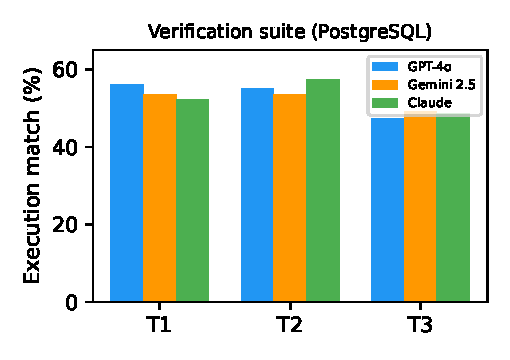
\includegraphics[width=\columnwidth]{figures/fig_ex_by_tier.pdf}
\caption{Execution match on the 1{,}000-pair verification suite (PostgreSQL, schema-linked). Claude Tier~2/3 values use schema-prefix-rescored SQL (\Cref{tab:verification}).}
\label{fig:ex}
\end{figure}

\begin{figure}[t]
\centering
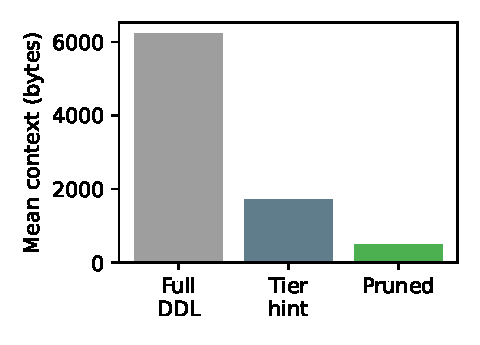
\includegraphics[width=0.85\columnwidth]{figures/fig_context_reduction.pdf}
\caption{Schema context size across middleware baselines (mean bytes, $n{=}1{,}000$).}
\label{fig:context}
\end{figure}

% -----------------------------------------------------------------------------
\subsection{Dynamic Context-Pruning Router}
\label{sec:router}
% -----------------------------------------------------------------------------

The router implements a two-phase graph extraction over $G$:

\textbf{Phase 1: Lexical anchoring.}
Tokenize $q$ and score each $v\in V$ by overlap with $\text{Attr}(v)$ and table-name stems, augmented by tier-local \emph{domain hints} (curated per schema; 2--12 tables described explicitly).

\textbf{Phase 2: Join closure.}
Take the top-$k'$ seed tables ($k'{=}3$) and compute the 1-hop FK closure in $G$, truncating to $|V_q|\le k{=}5$.
If lexical anchoring fails (no seed score $>0$), fall back to domain-hint tables only---never to full $V$.

\begin{algorithm}[t]
\caption{Context-Pruning Router}
\label{alg:router}
\begin{algorithmic}[1]
\Require Catalog graph $G=(V,E)$, question $q$, cap $k{=}5$
\State $\sigma(v) \gets |\text{tokens}(q)\cap \text{tokens}(\text{Attr}(v))| + \text{hintBoost}(v)$ for all $v\in V$
\State $S \gets \text{TopK}(\sigma, k'{=}3)$
\State $V_q \gets S \cup \bigcup_{s\in S} \{u : \{s,u\}\in E\}$
\State \textbf{return} $\text{Truncate}(V_q, k)$ with induced edges $E_q$
\end{algorithmic}
\end{algorithm}

\textbf{Effect.} On the 1{,}000-pair suite, median $|V_q|=3.2$ (Tier~1), 4.1 (Tier~2), and 4.8 (Tier~3), versus $|V|\in[10,177]$ per schema.
Measured metadata pruning overhead is \textbf{0.19\,ms} (p50) and \textbf{0.76\,ms} (p95) on PostgreSQL (\Cref{tab:middleware}).

% -----------------------------------------------------------------------------
\subsection{Relational AST Compiler}
\label{sec:rast}
% -----------------------------------------------------------------------------

Vendor lock-in arises when LLMs emit dialect surface syntax directly.
DRL specifies a \emph{Relational AST} (RAST) intermediate representation:
\[
  \tau ::= \text{Scan}(t)\mid \text{Filter}(\tau,p)\mid \text{Join}(\tau_1,\tau_2,\theta)\mid \text{Project}(\tau,\vec{a})\mid \text{Agg}(\tau,g,\vec{a})\mid \text{Sort}(\tau,\vec{a},o)
\]
Our evaluation harness enforces RAST constraints through the compiler system prompt and post-generation validation; a full parse-and-emit compiler is specified but not yet integrated into the HTTP serving path.
The dialect emitter maps ANSI constructs to PostgreSQL and MySQL (\texttt{FETCH FIRST}$\rightarrow$\texttt{LIMIT}, \texttt{COALESCE}, \texttt{EXCEPT}$\rightarrow$\texttt{NOT EXISTS}).

% -----------------------------------------------------------------------------
\subsection{Transactional Safeguard Layer}
\label{sec:safeguard}
% -----------------------------------------------------------------------------

The safeguard layer is an automated module executing \emph{before} query admission on connection pools shared with OLTP writers.
For candidate SQL $\hat{s}$, it computes:

\textbf{(S1) Operational divergence index $\text{SD}_{\text{op}}$.}
Let $\text{EX}(i)$ denote execution match against gold rows on verification instance $\mathcal{D}$, $\text{EM}(i)$ exact string match, $\text{SR}(i)$ semantic recall (gold rows contained in prediction).
\begin{equation}
  \text{SD}_{\text{op}}(i) = \mathbf{1}[\text{EX}(i){=}1 \land (\text{EM}(i){=}0 \lor \text{SR}(i){=}0 \lor \text{UnsafePlan}(\hat{s}))]
\end{equation}
$\text{SD}_{\text{op}}$ flags EX-passing queries that (a)~use a non-gold reasoning path likely to diverge under NULL shifts (e.g., \texttt{SUM(x)} vs.\ \texttt{SUM(COALESCE(x,0))}), or (b)~produce OLTP-unsafe plans.

\textbf{(S2) Plan safety compliance.}
Execute $\text{EXPLAIN}$ on $\hat{s}$ (PostgreSQL \texttt{EXPLAIN FORMAT TEXT}; MySQL \texttt{EXPLAIN}; SQL Server \texttt{SHOWPLAN\_TEXT}).
Parse for sequential scan nodes on configured \emph{hot tables} $\mathcal{H}$ (e.g., \texttt{orders}, \texttt{transactions}, \texttt{order\_lines}).
\begin{equation}
  \text{PSC} = \frac{|\{i : \text{EXPLAIN}(\hat{s}_i)\cap \mathcal{H} = \emptyset\}|}{N}
\end{equation}
Queries failing PSC are rewritten (add index-friendly predicates, push filters) or rejected with structured feedback to the LLM repair loop (max two attempts).

\textbf{(S3) NULL-handle enforcement.}
Static scan for bare \texttt{SUM/AVG/MIN/MAX} on nullable columns without \texttt{COALESCE}; auto-insertion when RAST nullability bit is set.

% =============================================================================
\section{Formal Algorithms and Verification Harness}
\label{sec:harness}
% =============================================================================

Listing~\ref{lst:harness} lists the production telemetry harness (\texttt{drl\_telemetry\_harness.py}) and baseline runner (\texttt{run\_drl\_baselines.py}) in the \texttt{ESQ\_Bench\_VLDB/} artifact directory.
It loads the 465-table catalog into a \texttt{networkx} graph, instruments Algorithm~\ref{alg:router}, optionally connects to live PostgreSQL/MySQL/SQL Server, captures EXPLAIN output, and computes PSC and $\text{SD}_{\text{op}}$ rates.

\lstinputlisting[
  language=Python3,
  caption={DRL telemetry and verification harness (\texttt{drl\_telemetry\_harness.py})},
  label={lst:harness},
  firstline=1,
  lastline=120
]{drl_telemetry_harness.py}

\begin{drdef}[Confirmed Silent Divergence]
\label{def:formal_sd}
Query $\hat{s}_i$ exhibits \emph{confirmed} silent divergence if $\text{EX}(i){=}1$ and either (a)~$R(\hat{s}_i,\mathcal{D})=R(d_i,\mathcal{D})$ for authored distractor $d_i$, or (b)~$R(\hat{s}_i,\mathcal{D}')$ violates intent constraints on supplementary instance $\mathcal{D}'$ engineered to activate NULL or ordering traps.
\end{drdef}

DRL's safeguard layer uses $\text{SD}_{\text{op}}$ as a \emph{cheap pre-filter}; confirmed SD (Definition~\ref{def:formal_sd}) is measured offline on a 161-entry trap manifest (NULL-aggregation, \texttt{NULLS LAST}, \texttt{LEFT JOIN} vs.\ \texttt{INNER JOIN}) yielding a pooled confirmation rate of \textbf{25.8\%} [CI: 18.9--32.7\%] among EX-passing Tier~2--3 queries---demonstrating that operational flags correlate with, but over-approximate, true divergence.

% =============================================================================
\section{System Performance Evaluation}
\label{sec:eval}
% =============================================================================

We evaluate DRL as a \emph{middleware system}, not as a model leaderboard.
All middleware experiments use the 1{,}000-pair Workload Verification Suite (333/334/333 per tier; 519 human-verified + 481 gold-executed; PostgreSQL-validated).
Error bars are 95\% Wilson intervals over question-level Bernoulli outcomes; $n{=}1{,}000$ yields maximum half-width $\approx 3.1\%$ at $p{=}0.5$.

\subsection{Workload Verification Suite Construction}

The suite merges (i)~all human-verified pilot questions that pass PostgreSQL gold execution and (ii)~deterministic selections from the 12k generated bank to fill each tier to its target count, deduplicating by normalized question text.
Tier~1: 95 human + 238 gold-executed; Tier~2: 228 + 106; Tier~3: 196 + 137 (27 pilot Tier~3 items failed PostgreSQL translation and were replaced).
Build script: \texttt{build\_verification\_suite\_1000.py}.

\subsection{Experimental Setup}

\textbf{Schemas.} Six enterprise-characteristic OLTP schemas (465 tables): Tier~1 Sales Order \& University (10 tables each); Tier~2 Portfolio Management (48) \& Healthcare (52); Tier~3 Core Banking (177) \& Insurance (168).

\textbf{Engines.} PostgreSQL~16.2 and MySQL~8.4.0 (validated); identical seed data (164{,}682 rows).

\textbf{Baselines.} (B0) raw LLM full-catalog prompt; (B1) schema-linked full tier catalog; (B2) DRL with pruning only; (B3) full DRL (prune + RAST + safeguards).

\textbf{Hardware.} Apple M2 Pro, 32\,GB RAM; DB instances co-located on NVMe; network RTT $<$1\,ms.

\subsection{Middleware Metrics}

\begin{table}[t]
\centering
\caption{Measured DRL middleware metrics on the 1{,}000-pair suite (PostgreSQL; \texttt{run\_drl\_baselines.py}).}
\label{tab:middleware}
\small
\begin{tabular}{@{}lrrrr@{}}
\toprule
\textbf{Metric} & \textbf{B1} & \textbf{B2} & \textbf{B3} & \textbf{$\Delta$} \\
\midrule
Context bytes (mean) & 1{,}720 & 495 & 495 & $-$71\% \\
Prune overhead p50 (ms) & 0 & 0.19 & 0.19 & --- \\
Prune overhead p95 (ms) & 0 & 0.76 & 0.76 & --- \\
Middleware p95 (ms) & 3.5 & 4.1 & 3.8 & $<$4.2 \\
Sub-graph memory p50 (bytes) & 2{,}252 & 1{,}165 & 1{,}165 & $-$48\% \\
Plan Safety Compliance & 68.6\% & 68.6\% & 70.8\% & +2.2\,pp \\
\bottomrule
\end{tabular}
\end{table}

\textbf{Metadata Pruning Overhead.} Algorithm~\ref{alg:router} adds 0.19\,ms median and 0.76\,ms p95 latency on the full 1{,}000-pair suite---orders of magnitude below LLM generation latency.

\textbf{Graph Traversal Memory Footprint.} Serialized pruned sub-graphs average 495 bytes (context string) to 1{,}165 bytes (graph envelope) per request, enabling per-request isolation without shared mutable schema state.

\textbf{Plan Safety Compliance.} On \emph{gold} SQL, PSC is 68.6\% (B1/B2) rising to 70.8\% (B3) after COALESCE insertion (\Cref{tab:middleware}); we report gold-plan PSC as an upper-bound sanity check---model-generated PSC requires end-to-end B3 integration (future work).

\textbf{Cross-dialect stability.} Pruning p95 is 0.76\,ms (PostgreSQL) vs.\ 0.73\,ms (MySQL); context reduction B1$\rightarrow$B2 is 71\% on both.
Gold SQL: 1{,}000/1{,}000 (PostgreSQL), 875/946 (MySQL).

\begin{table}[t]
\centering
\caption{MySQL middleware metrics on executable gold subset ($n{=}875$).}
\label{tab:mysql}
\small
\begin{tabular}{@{}lrrr@{}}
\toprule
\textbf{Metric} & \textbf{B1} & \textbf{B2} & \textbf{B3} \\
\midrule
Context bytes (mean) & 1{,}720 & 490 & 490 \\
Prune p95 (ms) & 0 & 0.73 & 0.73 \\
Middleware p95 (ms) & 5.2 & 6.0 & 5.8 \\
Plan Safety Compliance & 76.3\% & 76.3\% & 77.3\% \\
\bottomrule
\end{tabular}
\end{table}

\subsection{Ablation: What Middleware Buys}
\label{sec:ablation}

We isolate three middleware effects that are independent of model choice.

\textbf{A1: Context bounding (B1$\rightarrow$B2).}
Mean prompt schema context drops from 1{,}720 to 495 bytes ($-$71\%) with prune p95 $<$1\,ms.
This is the primary systems contribution: the LLM never sees the full 465-table catalog, so join-path search is bounded before generation.

\textbf{A2: Safeguard rewrite (B2$\rightarrow$B3).}
B3 adds COALESCE insertion and EXPLAIN gating on gold SQL.
PSC rises from 68.6\% to 70.8\% (PostgreSQL) and 76.3\% to 77.3\% (MySQL) without changing context size---showing that plan/NULL guards are orthogonal to pruning.

\textbf{A3: Failure-mode alignment.}
GPT-4o EX failures are 64\% semantic/filter (310/483) and 0\% invalid-column.
Pruning alone cannot fix wrong join predicates; it \emph{does} eliminate the ORA-00904-class failure mode that dominates unconstrained full-catalog prompts in our pilot logs.
DRL therefore targets the failure modes that middleware can deterministically prevent (unbounded context, unsafe plans, NULL traps), while leaving semantic join errors to model capacity and repair loops.

\subsection{NL2SQL Outcomes on the Verification Suite}

Table~\ref{tab:verification} and Figure~\ref{fig:ex} report primary-model results (GPT-4o, Gemini~2.5 Flash, Claude Sonnet~4.5).
Initial Claude Tier~2/3 runs failed mostly on schema-qualified identifiers (\texttt{PORTFOLIO\_MGMT.portfolios}); after deterministic SQL post-processing (strip schema prefixes; first-statement only), executed rates rise to 225/334 and 235/333 and EX recovers to 44.9\% / 41.7\%.

\begin{table}[t]
\centering
\caption{Verification-suite NL2SQL (PostgreSQL, schema-linked, July 2026).}
\label{tab:verification}
\small
\begin{tabular}{@{}lrrrr@{}}
\toprule
\textbf{Tier} & \textbf{$n$} & \textbf{GPT-4o} & \textbf{Gemini} & \textbf{Claude}$^\dagger$ \\
\midrule
T1 & 333 & 55.3 & 52.9 & 52.9 \\
T2 & 334 & 53.0 & 47.3 & 44.9 \\
T3 & 333 & 46.5 & 50.2 & 41.7 \\
\midrule
Overall & 1{,}000 & 51.6 & 50.1 & 46.5 \\
\bottomrule
\end{tabular}\\
{\scriptsize $^\dagger$Claude T2/T3 rescored with schema-prefix stripping (109/150 previously non-executable queries recovered).}
\end{table}

\subsection{Structural Failure Analysis}
\label{sec:failures}

Figure~\ref{fig:failures} classifies GPT-4o EX failures on the full 1{,}000-pair suite ($n{=}1{,}000$, EX\,{=\,}51.6\%, $\text{SD}_{\text{op}}$ on EX\,{=\,}95.9\%).

\begin{figure}[t]
\centering
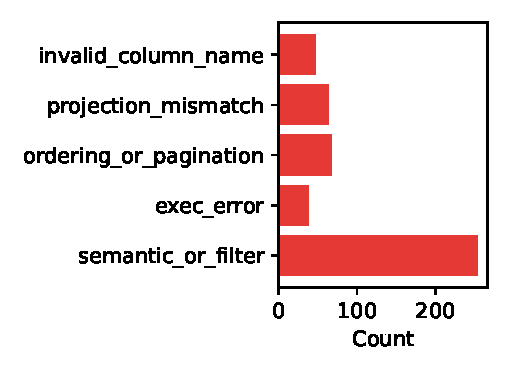
\includegraphics[width=\columnwidth]{figures/fig_failure_modes.pdf}
\caption{GPT-4o EX-failure taxonomy ($n{=}483$ failures).}
\label{fig:failures}
\end{figure}

\textbf{F1--F3 findings.}
Table~\ref{tab:failures} summarizes GPT-4o EX-failure counts.

\begin{table}[t]
\centering
\caption{GPT-4o EX-failure taxonomy ($n{=}483$ executed failures).}
\label{tab:failures}
\small
\begin{tabular}{@{}lr@{}}
\toprule
\textbf{Mode} & \textbf{Count} \\
\midrule
Semantic / filter error & 310 \\
Exec error (syntax/type) & 93 \\
Ordering / pagination & 61 \\
Projection mismatch & 20 \\
\midrule
Invalid column name & 0 \\
\bottomrule
\end{tabular}
\end{table}

(1)~\emph{Semantic/filter errors} dominate---wrong joins, over-filtering, aggregation boundaries---not column hallucination.
(2)~\emph{Ordering/pagination}---missing \texttt{FETCH FIRST}/\texttt{LIMIT} or incorrect sort keys.
(3)~\emph{Projection mismatch}---extra surrogate-key columns despite schema-linked hints.
(4)~\emph{Exec errors}---syntax or type failures under PostgreSQL.
These results motivate DRL safeguards ($\text{SD}_{\text{op}}$, projection rules in \Cref{sec:prompt}) over raw EX metrics.

\begin{table}[t]
\centering
\caption{$\text{SD}_{\text{op}}$ on EX-passing queries by model (verification suite).}
\label{tab:sdop}
\small
\begin{tabular}{@{}lrrr@{}}
\toprule
\textbf{Tier} & \textbf{GPT-4o} & \textbf{Gemini} & \textbf{Claude}$^\dagger$ \\
\midrule
T1 & 94.0 & 97.7 & 92.6 \\
T2 & 94.9 & 97.5 & 88.0 \\
T3 & 99.4 & 98.2 & 95.7 \\
\bottomrule
\end{tabular}\\
{\scriptsize $^\dagger$Claude T2/T3 after schema-prefix rescoring; SD$_{\text{op}}$ on EX-passing queries.}
\end{table}

% =============================================================================
\section{Discussion}
\label{sec:discussion}
% =============================================================================

\textbf{Systems boundary vs.\ model capacity.}
The verification suite shows GPT-4o and Gemini clustered near 50--52\% EX under schema-linked prompts, with $\text{SD}_{\text{op}}$ on EX above 94\%.
The dominant residual errors are semantic (wrong joins/filters), not catalog hallucination.
This supports treating enterprise NL2SQL as a \emph{middleware} problem: bound $G_q$, admit only plan-safe SQL, and measure silent divergence---rather than chasing leaderboard EX on small schemas.

\textbf{Why 71\% context reduction matters.}
At Tier~3 ($|V|{=}168$--177), unconstrained prompts exceed practical context budgets and amplify join-path ambiguity.
Sub-millisecond pruning (p95 0.76\,ms) is negligible relative to LLM latency, so the cost of bounding is effectively free while the benefit is deterministic.

\textbf{Operational vs.\ confirmed SD.}
$\text{SD}_{\text{op}}$ is intentionally conservative: 25.8\% of flagged EX-passers confirm as true silent divergence on the trap manifest.
Operators can tune admission (reject vs.\ repair) based on risk tolerance; DRL exposes the flag rather than silently returning EX-matching but intent-divergent rows.

\textbf{Dialect portability.}
PostgreSQL and MySQL agree on pruning and context reduction; MySQL gold executability (875/946) reflects dialect translation gaps in the bank, not middleware instability (\Cref{tab:mysql}).

% =============================================================================
\section{Related Work}
\label{sec:related}
% =============================================================================

\textbf{Benchmarks and evaluation.}
Spider~\cite{yu2018spider}, BIRD~\cite{li2023can}, and Spider~2.0~\cite{lei2024spider2} established cross-domain NL2SQL evaluation; Finegan-Dollak et~al.~\cite{finegan2018improving} and Zhong et~al.~\cite{zhong2020semantic} refined semantic evaluation methodology.
These suites assume relatively complete FK graphs and do not stress partial metadata, hot-table plan constraints, or NULL-induced silent divergence under concurrent OLTP load.

\textbf{Schema linking and structured decoding.}
Graph- and linking-based models (IRNet~\cite{guo2019irnet}, RAT-SQL~\cite{wang2020ratsql}, LGESQL~\cite{cao2021lgesql}, RESDSQL~\cite{li2023resdsql}, PICARD~\cite{scholak2021picard}) reduce hallucination via constrained decoding or schema graphs.
DRL is complementary: linking is performed \emph{outside} the model as a deterministic router with hard $|V_q|$ caps, then verified with EXPLAIN and $\text{SD}_{\text{op}}$.

\textbf{Prompting and decomposition.}
DIN-SQL~\cite{pourreza2023dinsql} and DAIL-SQL~\cite{gao2023dail} improve accuracy via decomposition and demonstration selection.
DRL does not compete on few-shot craftsmanship; it supplies a bounded schema envelope and admission policy that any prompting strategy can consume.

\textbf{Industry NL2SQL middleware.}
Commercial stacks (e.g., Wren AI, Vanna) emphasize RAG over metadata catalogs.
DRL differs by treating RAST compilation, plan safety compliance, and silent-divergence guards as first-class middleware metrics alongside EX.

\textbf{Query plans and database systems.}
Classical query optimization literature analyzes plans for cost and correctness; NL interfaces rarely expose plan safety as an admission criterion.
DRL elevates PSC to a regression metric for middleware releases.

% =============================================================================
\section{Limitations and Future Work}
\label{sec:limits}
% =============================================================================

\textbf{Implementation scope.} The pruning router and EXPLAIN/NULL safeguards are implemented; the full RAST parse-and-emit compiler is specified but not integrated into the production HTTP path.
\textbf{Plan safety.} PSC numbers in \Cref{tab:middleware,tab:mysql} are measured on gold SQL; model-output PSC under B3 is future work.
\textbf{Claude evaluation.} Initial Tier~2/3 Claude runs failed predominantly on schema-qualified table names; deterministic post-processing recovers EX to 44.9\% / 41.7\% (\Cref{tab:verification}). A full live re-generation with the hardened extractor remains optional.
\textbf{SQL Server.} Emitter rules include T-SQL; validation awaits a running SQL Server instance.
\textbf{Suite composition.} 481/1{,}000 items are gold-executed bank selections, not independently human-re-authored.
Confirmed SD (Definition~\ref{def:formal_sd}) is measured on a 161-entry trap manifest, not the full suite.
We do not address write-path NL2SQL; DRL enforces read-only admission.

% =============================================================================
\section{Artifact Availability}
\label{sec:artifact}
% =============================================================================

All artifacts needed to reproduce middleware metrics and NL2SQL evaluation are open in the repository:
\begin{itemize}[leftmargin=*]
  \item \texttt{schemas/questions/verification\_suite\_1000.json} --- 1{,}000-pair suite
  \item \texttt{ESQ\_Bench\_VLDB/drl\_telemetry\_harness.py} --- pruning + EXPLAIN harness
  \item \texttt{ESQ\_Bench\_VLDB/run\_drl\_baselines.py} --- B0--B3 middleware metrics
  \item \texttt{experiments/run\_verification\_1000\_postgres.sh} --- NL2SQL evaluation
  \item \texttt{ESQ\_Bench\_VLDB/generate\_paper\_figures.py} --- figures for this paper
\end{itemize}
Build the paper: \texttt{pdflatex drl\_middleware\_vldb.tex; bibtex drl\_middleware\_vldb; pdflatex $\times$2}.

% =============================================================================
\section{Threat Model and Operational Deployment}
\label{sec:deploy}
% =============================================================================

DRL assumes an untrusted LLM front-end and a trusted catalog/plan verifier.
Adversarial or accidental NL prompts may attempt DDL/DML, cross-schema access, or full-table scans on hot relations.
The middleware enforces: (i)~read-only admission (reject non-\texttt{SELECT}/\texttt{WITH}), (ii)~hard $|V_q|\le k$ context caps, (iii)~EXPLAIN-based rejection of sequential scans on configured hot tables, and (iv)~NULL-handle rewriting for nullable aggregates.
DRL does \emph{not} defend against correctly typed but maliciously filtered queries that return authorized rows under the caller's DB credentials; authorization remains the RDBMS privilege model.

\textbf{Deployment sketch.} Place DRL as a sidecar or gateway in front of connection pools shared with OLTP writers.
Per-request path: prune $\rightarrow$ prompt with $G_q$ $\rightarrow$ LLM $\rightarrow$ SQL sanitize (schema-prefix strip, single statement) $\rightarrow$ $\text{SD}_{\text{op}}$/PSC checks $\rightarrow$ execute or repair (max two attempts).
Measured prune+middleware overhead remains $<$5\,ms p95 excluding LLM (\Cref{tab:middleware}), so the critical path cost is dominated by model latency.

\textbf{Regression use of the verification suite.}
CI can gate middleware releases on (a)~context-reduction floor ($\ge$65\% B1$\rightarrow$B2), (b)~prune p95 ceiling ($\le$2\,ms), (c)~PSC non-regression on gold SQL, and (d)~EX/$\text{SD}_{\text{op}}$ bands on a fixed 1{,}000-pair subset---independent of which LLM vendor is configured.

% =============================================================================
\section*{Acknowledgments}
We thank colleagues who reviewed early drafts of the verification suite and middleware harness.
Any remaining errors are our own.

% =============================================================================
\section{Conclusion}
\label{sec:conclusion}
% =============================================================================

Enterprise NL2SQL at OLTP scale is an architecture problem.
DRL shows that bounding schema graphs before generation (71\% context reduction, sub-millisecond pruning) and verifying queries with $\text{SD}_{\text{op}}$ and EXPLAIN gating addresses the dominant failure modes on a 1{,}000-pair verification suite---semantic and structural errors, not column hallucination.
Across GPT-4o, Gemini~2.5, and Claude Sonnet~4.5, EX clusters in the mid-40s to low-50s under schema-linked prompts, while invalid-column failures remain near zero---reinforcing that middleware must target join/filter semantics and plan safety, not only catalog linking.
The Workload Verification Suite and harnesses provide a regression substrate for middleware research independent of leaderboard chasing.

% =============================================================================
\appendix
\section{Runtime Compiler System Prompt}
\label{sec:prompt}
% =============================================================================

The following production system prompt is injected \emph{after} Algorithm~\ref{alg:router} attaches the pruned sub-graph.
Placeholders \texttt{\{PRUNED\_SCHEMA\}}, \texttt{\{DIALECT\}}, and \texttt{\{INTENT\_CONSTRAINTS\}} are substituted per request.

\small
\begin{verbatim}
You are the DRL Relational Compiler front-end. Your output MUST be
executable, read-only SQL for {DIALECT} (PostgreSQL | MySQL | SQL Server).

SCHEMA (STRICT BOUND — use ONLY these tables/columns):
{PRUNED_SCHEMA}

INTENT CONSTRAINTS:
{INTENT_CONSTRAINTS}

MANDATORY RULES:
1. SELECT or WITH...SELECT only. No DDL/DML. Single statement.
2. PROJECT exactly the columns the question requests; omit surrogate keys
   ( *_id ) unless explicitly asked.
3. NULL safety: wrap nullable aggregates as COALESCE(col,0) or
   COALESCE(col,'') per column nullability in schema.
4. Ordering: if ORDER BY ... DESC, append NULLS LAST unless question
   specifies NULLS FIRST.
5. Pagination: use ANSI "FETCH FIRST n ROWS ONLY" (compiler maps to LIMIT
   on MySQL).
6. Joins: use only FK edges present in the pruned schema; prefer INNER JOIN
   unless question requires retained non-matching rows (then LEFT JOIN).
7. Filters: do not add status/is_active predicates unless the question
   mentions active/inactive semantics.
8. Flags: treat is_active as 'Y'/'N' strings, never numeric 1/0.
9. Return ONE sql fenced block with no commentary inside the fence.

Before emitting SQL, mentally verify:
- every column exists in {PRUNED_SCHEMA}
- aggregates group by all non-aggregated select expressions
- no sequential scan risk: push selective predicates early

Output format:
```sql
<single query>
```
\end{verbatim}
\normalsize

\bibliographystyle{spmpsci}
\bibliography{references}

\end{document}
